\chapter{\resultsname}
\label{chap:resultados}

Se ejecutaron 24 casos (6 proyectos $\times$ 4 flujos) mediante scripts automatizados sobre entornos aislados. Todas las ejecuciones se completaron. En Authentik, C0 gener\'o una funcionalidad distinta a la solicitada (SCIM provisioning donde se ped\'ia una correcci\'on de compatibilidad FIPS), lo que muestra que sin una especificaci\'on clara el agente puede interpretar incorrectamente el objetivo.

\section{Evaluaci\'on autom\'atica de calidad de c\'odigo}

\begin{table}[htbp]
\centering
\caption{An\'alisis autom\'atico: hallazgos clave}
\label{tab:auto-resumen}
\begin{tabularx}{\textwidth}{lX}
\toprule
\textbf{Herramienta} & \textbf{Hallazgo} \\
\midrule
\texttt{semgrep} & 1 issue de seguridad (ReDoS en C0 Directus). C\'odigo limpio de bugs en general. \\
\texttt{eslint} & 2--74 incidencias por caso. M\'as incidencias donde hay m\'as TypeScript. \\
\texttt{phpcs} & \textbf{16.009 incidencias en C0 Appwrite} vs. \textbf{1.597 en C1} ($-$90\%). \\
\texttt{shellcheck} & 12 incidencias est\'andar en C0--C2 (boilerplate SpecKit). \\
\texttt{pyflakes} & 0--1 incidencias. C\'odigo Python limpio. \\
\texttt{cloc} & C2 genera m\'as l\'ineas (14.218) que C0 (5.948) por incluir tests y documentaci\'on. \\
\bottomrule
\end{tabularx}
\end{table}

\begin{table}[htbp]
\centering
\caption{Incidencias \texttt{phpcs}: Appwrite (10832)}
\label{tab:phpcs}
\begin{tabular}{lcc}
\toprule
\textbf{Flujo} & \textbf{Incidencias} & \textbf{vs.\ C0} \\
\midrule
C0 & 16.009 & --- \\
C1 & \textbf{1.597} & \textbf{$-$90\%} \\
C2 & 14.577 & $-$9\% \\
C3 & 326 & $-$98\% (c\'odigo m\'inimo) \\
\bottomrule
\end{tabular}
\end{table}

\FloatBarrier
\section{Evaluaci\'on manual: r\'ubrica SRCI v3}

\begin{table}[htbp]
\centering
\caption{Evaluaci\'on SRCI v3: notas globales /10}
\label{tab:srci-global}
\begin{tabular}{lccccc}
\toprule
\textbf{Flujo} & \textbf{A (/12)} & \textbf{B (/5)} & \textbf{C (/3)} & \textbf{TSR} & \textbf{Nota/10} \\
\midrule
C0 SpecKit vanilla   & 3.0 & 3.9 & 0.3 & 0.92 & 6.3 \\
C1 IREB v1           & 3.2 & 4.0 & 0.7 & 1.00 & 6.8 \\
C2 IREB v2           & 3.2 & 4.0 & 1.7 & 1.00 & 7.2 \\
C3 MRS directo       & 3.0 & 3.6 & 0.0 & 0.17 & 2.8 \\
\bottomrule
\end{tabular}
\end{table}

La progresi\'on C3 (2.8) $\rightarrow$ C0 (6.3) $\rightarrow$ C1 (6.8) $\rightarrow$ C2 (7.2) muestra que cada paso a\~nadido mejora el resultado: el pipeline m\'inimo (+3.5 puntos), la formalizaci\'on IREB (+0.5), los mecanismos de robustez (+0.4). Por bloques, la formalizaci\'on IREB (C0 $\rightarrow$ C1) mejora la conformidad de la implementaci\'on (Bloque B: 3.9 $\rightarrow$ 4.0) y eleva el TSR al 100\,\%. El \emph{scope contract} y \texttt{AGENTS.md} (C1 $\rightarrow$ C2) concentran su efecto en la verificaci\'on: C2 es el \'unico flujo que genera tests en los 6 casos.

\FloatBarrier
\section{An\'alisis de coste}

\begin{table}[htbp]
\centering
\caption{Coste monetario por flujo (media de 6 casos)}
\label{tab:coste-real}
\begin{tabular}{lccc}
\toprule
\textbf{Flujo} & \textbf{Coste medio} & \textbf{Nota/10} & \textbf{Eficiencia (pts/\$)} \\
\midrule
C0 & \$0.0407 & 6.3 & 155 \\
C1 & \$0.0608 & 6.8 & 112 \\
C2 & \$0.0696 & 7.2 & 103 \\
C3 & \$0.0115 & 2.8 & 243 \\
\bottomrule
\end{tabular}
\end{table}

El coste crece con la calidad: C2 cuesta un 71\,\% m\'as que C0, pero es el \'unico flujo con tests en todos los casos. C3 es la opci\'on m\'as econ\'omica, aunque su capacidad para implementar requisitos reales es limitada (TSR del 17\,\%).

\section{Visualizaci\'on comparativa}

\begin{figure}[htbp]
\centering
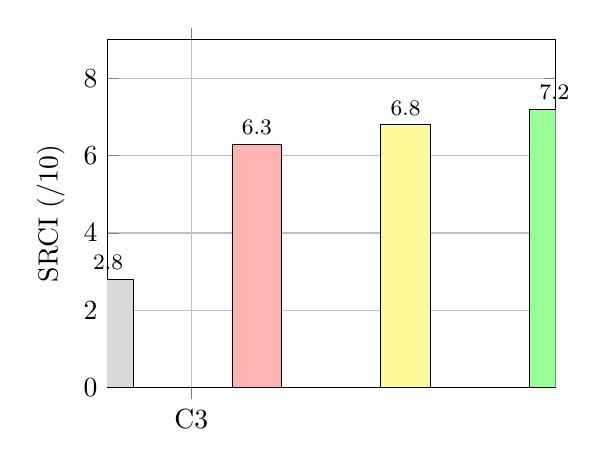
\begin{tikzpicture}
\begin{axis}[
    ybar,
    bar width=18pt,
    width=0.6\textwidth,
    height=6cm,
    ylabel={SRCI (/10)},
    ymin=0, ymax=9,
    xtick=data,
    xticklabels={C3, C0, C1, C2},
    enlarge x limits=0.3,
    grid=major,
    nodes near coords,
    every node near coord/.append style={font=\footnotesize}
]
\addplot[fill=gray!30]   coordinates {(1,2.8)};
\addplot[fill=red!30]    coordinates {(2,6.3)};
\addplot[fill=yellow!40] coordinates {(3,6.8)};
\addplot[fill=green!40]  coordinates {(4,7.2)};
\end{axis}
\end{tikzpicture}
\caption{Puntuaci\'on SRCI media de cada condici\'on experimental (media de 6 casos).}
\label{fig:barras-4flujos}
\end{figure}

\section{Resumen de m\'etricas}

\begin{table}[htbp]
\centering
\caption{Tabla resumen de todas las m\'etricas por flujo}
\label{tab:resumen-metricas}
\begin{tabular}{lcccc}
\toprule
\textbf{M\'etrica} & \textbf{C0} & \textbf{C1} & \textbf{C2} & \textbf{C3} \\
\midrule
SRCI (/10) & 6.3 & 6.8 & \textbf{7.2} & 2.8 \\
TSR (\%) & 92 & \textbf{100} & \textbf{100} & 17 \\
Tests (casos con tests) & 1/6 & 3/6 & \textbf{6/6} & 0/6 \\
Coste medio (\$) & 0.0407 & 0.0608 & 0.0696 & \textbf{0.0115} \\
L\'ineas c\'odigo (media) & 5.948 & 18.522 & 14.218 & \textbf{289} \\
\midrule
\textbf{Eficiencia (pts/\$)} & 155 & 112 & 103 & \textbf{243} \\
\bottomrule
\end{tabular}
\end{table}